% This is the template I use for all my college work 
% No frills, no nonsense and optimized for readability and compactness
% You can easily slap on additional features

\documentclass[11pt,a4paper]{article}
\usepackage[margin=0.6in]{geometry}
% if your work is to be printed and filed, consider 1 in margins
\usepackage[utf8]{inputenc}
% change 'inputenc' to 'ctexart' to enable chinese

\usepackage{amsmath, amsthm, amssymb, fancyhdr, pgfplots, enumerate, graphicx}
% amsmath   - extra features for typing math
% amsthm    - defines theorem structures (theorem, proof, etc.)
% amssymb   - math symbols and math fonts (notably mathbb and mathcal)
% fancyhdr  - nice looking header/footers
% pgfplots  - plotting graphs
% enumerate - allows to changing style of enumeration easily e.g. a) b) c) (i) (ii) (iii)
% graphic   - adding images to your document

\pgfplotsset{compat=1.14}
% Setting backwards compatibility to enable pgfplot settings
\usepgfplotslibrary{fillbetween}
% Useful feature when shading graphs 

\newtheorem{theorem}{Theorem}
\newtheorem{lem}{Lemma}
% Custom defined theorem environments (commonly used)

\newcommand{\hwnum}{1}
\newcommand{\coursenum}{12-345}
\newcounter{problem}

\newcommand\Problem{
  \stepcounter{problem}
  {\large \textbf{Problem \theproblem.}~}
}

\fancyfoot[L]{Yang Gan}
\fancyfoot[C]{\small \LaTeX Crash Course}
\fancyfoot[R]{\thepage}
\renewcommand\headrulewidth{0pt}
\pagestyle{fancy}

\begin{document}
\textbf{\coursenum \ HW\hwnum \hfill \today}\\
\noindent\rule{\textwidth}{1pt} \\
\Problem 
In \LaTeX, normal text is compiled in the same font. It is also space insensitive, which means that any amount of blank space
is
        treated
                as a single
                        space. \\
There are many ways to start a new paragraph. This is without indent. \\
\par
This is with an indent. \\\\
I usually use this. \\\\
\textbf{Basic typesetting}
\begin{enumerate}
    \item 
    Item 1
    \begin{enumerate}
        \item 
        Sub-item 1
    \end{enumerate}
    \item
    Item 2
\end{enumerate}
After enumeration you will automatically be put in a new paragraph (with indents). \\\\
\textbf{This is bold}\\\\
\textit{This is italicized}\\\\
\underline{This is underlined}
\begin{enumerate}[a)]
    \item
    We can use options to redefine enumeration style
    
    \item
    You can also try other options like [i)], [a.], [(i)], etc.
\end{enumerate}
\noindent If you don't want indents after enumeration, you need to do this. Next we explore itemize, which creates bullet point itemization. 
\begin{itemize}
    \item 
    Bullet point 1
    \begin{itemize}
        \item 
        Sub-bullet point 1
    \end{itemize}
    \item
    Bullet point 2
\end{itemize}
We can also make a table. We separate column entries with ampersand


\begin{figure}[h]
    \centering
    \begin{tabular}{c|c|c}
        8 & 1 & 6 \\
        \hline
        % separating rows with lines
        3 & 5 & 7 \\
        % no line here
        4 & 9 & 2
    \end{tabular}
    \caption{A Magic Square}
\end{figure}

You can also add diagonal slash boxes using the package \emph{diagbox}. You can research on how to do this, but I exclude it for most of my work because I don't need to draw many tables. 


% Lastly, this jumps to a new page
\pagebreak
\noindent\rule{\textwidth}{1pt} \\
\Problem \textbf{\large Math Mode} \\\\
There are two main kinds of math modes used, in-line style and equation mode. In-line math mode is achieved with the dollar sign, such as $x, y, z$. \\\\
Usually most things work as you would expect them to in math mode. Some characters have special uses, so you can try adding a backslash. For example, \$4, $\{a, b, c\}$. \\\\
Equation mode makes \LaTeX automatically format equations for you. They will be centralized, space will be automatically allocated and you will also get an equation number:
\begin{equation}
    a^2 + b^2 = c^2
\end{equation}
Using the starred versions of such environments will remove the equation numbering. You can also add custom tags as such:
\begin{equation*}
    a^2 + b^2 = c^2 \tag{Pythagoras Theorem}
\end{equation*}
Since the above is used so often, there is a shortcut, which is to use
\[
    y = 2x
\]
However, more commonly used is the \emph{align} environment, which allows you to align multiple equations using ampersand (and breaking new line with double backslash):
\begin{align*}
    f(x) =& 1/x \\
    =& 1 - (x-1) + (x-1)^2 - (x-1)^3 \\
    & + (x-1)^4 - ...
\end{align*}
Now we shall go through some common things you'd want to know. \\\\
\noindent\rule{\textwidth}{0.6pt} \\
{\large Superscript and subscript}
\begin{align*}
    f(x, a) &= a + (x - a)^2 + (x-1)^2a + x^{2a} \\
    g(\pmb{x}) &= \| x_1^2 + x_2^2 + ... + x_{n+1}^2 \|
\end{align*}

\noindent\rule{\textwidth}{0.6pt} \\
{\large Fractions and Combination}
\begin{align*}
    2 &= 1 + \frac{1}{2} + \frac{1}{4} + \frac{1}{8} + ... \\
    \frac{dy}{dx} &= \frac{1}{x} \\[7pt]
    % need a bit more space here
    \binom{n}{k} &= \frac{n!}{k!\ (n-k)!}
\end{align*}
Often with fractions we will face the following problem:
\[
    (\frac{1}{2}x + y)^2 = \frac{1}{4}x^2 + xy + y^2
\]
The solution for all problems with bracket size can be resolved by using the left and right commands:
\[
    \left(\frac{1}{2}x + y \right)^2 = \frac{1}{4}x^2 + xy + y^2
\]
We can use that for other brackets as well:
\[
    \left\{\frac{1}{2}x + y \right\}^2 = \frac{1}{4}x^2 + xy + y^2
\]

\noindent\rule{\textwidth}{0.6pt} \\
{\large Sums, products, limits, integrals}
\begin{align*}
    \sum_{i = 1}^n i^2 &= \frac{n(n+1)(2n+1)}{6} \\[12pt]
    \frac{\pi}{2} &= \prod_{i = 1}^\infty \frac{4i^2}{4i^2 - 1} \\[12pt]
    e &= \lim_{n \to \infty} \left( 1 + \frac{1}{n} \right)^n \\[12pt]
    \sqrt{\pi} &= \int_{-\infty}^\infty e^{-x^2}\ dx
\end{align*}

\noindent\rule{\textwidth}{0.6pt} \\
{\large Case Environment}
\begin{align*}
    \theta(x) = \begin{cases}
        0 & \text{  if  $x < 0$} \\
        1 & \text{  if  $x \geq 0$}
    \end{cases}
\end{align*}

\noindent\rule{\textwidth}{0.6pt} \\
{\large Matrices}
\begin{align*}
    & A =
    \begin{pmatrix}
        -3 & 1 \\
        1  & 4
    \end{pmatrix}
    \begin{pmatrix}
        -7 & 0 \\
        0  & 6 
    \end{pmatrix}
    \begin{pmatrix}
        -\frac{4}{13}  &  \frac{1}{13} \\[6pt]
        \frac{1}{13}   &  \frac{3}{13}
    \end{pmatrix} = 
    \begin{pmatrix}
        -6 & 3 \\
        4 & 5
    \end{pmatrix} \\[12pt]
    \implies & \det (A - \lambda I) = (\lambda + 7)(\lambda - 6) \\
    \implies & \lambda_1 = -7,\ \lambda_2 = 6 \\[15pt] 
    & Ax = \lambda_1 x \implies x = t\begin{bmatrix}
        -3 \\
        1
    \end{bmatrix} \\
    & Ax = \lambda_2 x \implies x = t\begin{bmatrix}
        1 \\
        4
    \end{bmatrix}
\end{align*}

\noindent\rule{\textwidth}{0.6pt} \\
{\large Special Fonts \& Symbols}
\begin{align*}
    &\pm         \tag{``plus minus''} \\
    &\leq        \tag{``lesser or equal''} \\
    &\geq        \tag{``greater or equal''} \\
    &\neq        \tag{``not equal''} \\
    &\implies    \\
    &\impliedby  \\
    &\iff        \tag{``if and only if''} \\
    &\forall     \\
    &\exists
    &\in         \\
    &\subset, \subseteq         \tag{``subset or equal''} \\
    &\supset, \supseteq         \tag{``superset or equal''} \\
    &\cup, \cap \\
    &\mathbb{N}, \mathbb{Q}, \mathbb{R}, \mathbb{C}, \mathbb{E}, \mathbb{P}                  \tag{``Blackboard Bold''} \\
    &\mathcal{L}, \mathcal{P}   \tag{``Caligraphic''} \\
    &\alpha, \beta, \gamma, \delta, \epsilon, \zeta, \eta \dots
\end{align*}

\pagebreak
\noindent\rule{\textwidth}{1pt} \\
\Problem \textbf{\large Adding images}
\begin{figure}[hbt]
    \centering
    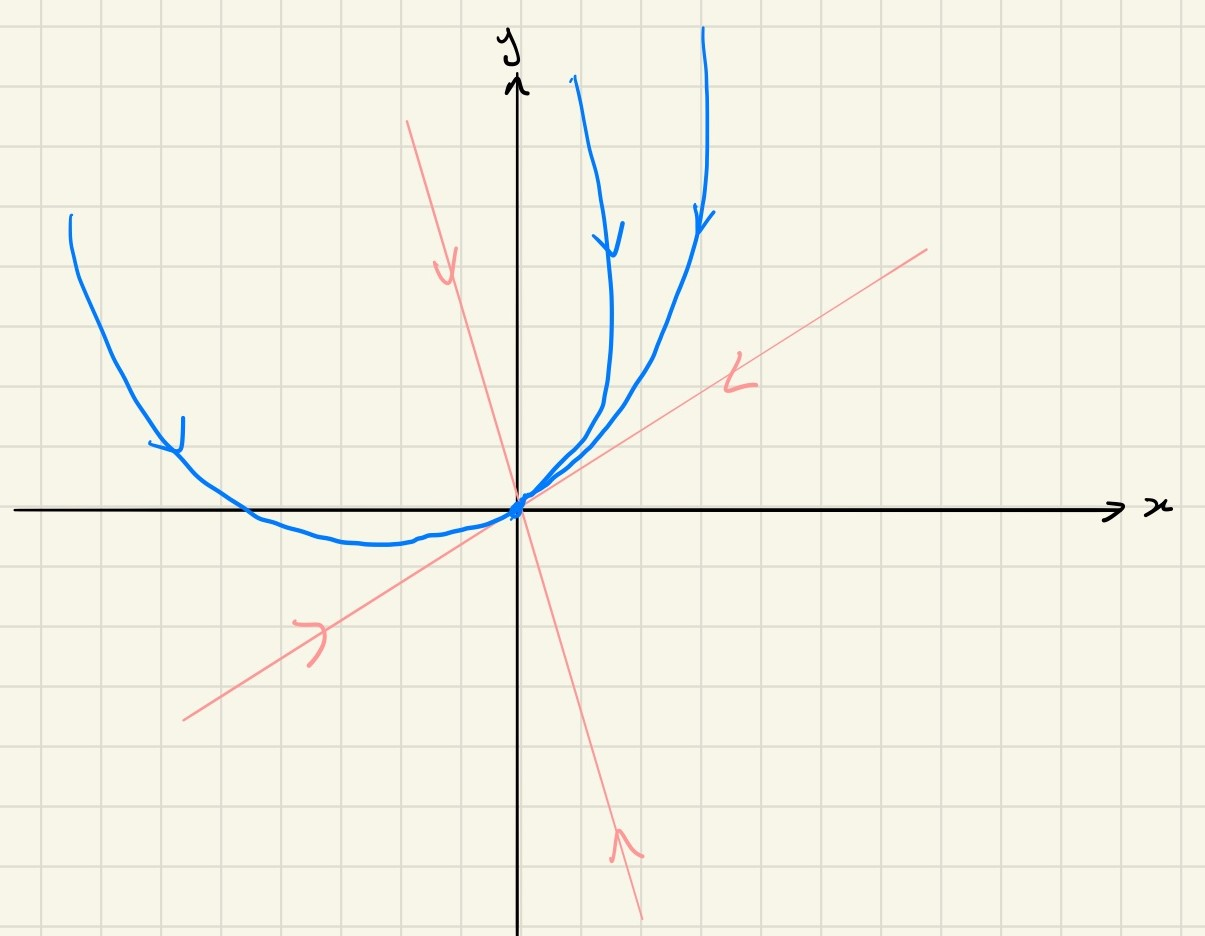
\includegraphics[width=.6\linewidth]{sampleimage.jpg}
    \caption{That's all!}
\end{figure}

\pagebreak
\noindent\rule{\textwidth}{1pt} \\
\Problem \textbf{\large Theorem Environment} \\\\
We can use the theorem environment to state and prove theorems neatly. 
\begin{theorem}
    For every odd $n$ we have
    \[
        n^2 \equiv 1 \mod 4
    \]
    
    \begin{proof}
        Letting $n = 2k$ for some $k\in \mathbb{Z}$ we have
        \begin{align*}
            n^2 &= (2k + 1)^2 \\
            &= 4k^2 + 4k + 1 \\
            &\equiv 1 \mod 4
        \end{align*}
    \end{proof}
\end{theorem}

\noindent \\
We can name our theorems and proofs as well.
\begin{theorem}[Fermat's Last Theorem]
    No three positive integers $a, b, c$ satisfy the equation
    \[
        a^n + b^n = c^n
    \]
    For integer $n > 2$.
    
    \begin{proof}[Proof by exercise]
        Left as an exercise to the reader.
    \end{proof}
\end{theorem}

\noindent \\
Notice that we have defined a lemma environment as well. It works exactly the same way.

\begin{lem}
    Let $x\in \mathbb{R}$ such that $x>0$, then we must have $\frac{1}{x} >0 $ as well.
    
    \begin{proof}
        Assume the contrary, then $\frac{1}{x} \leq 0$. Then we have
        \begin{align*}
            &-\frac{1}{x} \geq 0 \\
            \Rightarrow & (x)\cdot (-\frac{1}{x}) \geq 0 \\
            \Rightarrow & -(x\cdot \frac{1}{x}) \geq 0 \\
            \Rightarrow & -1 \geq 0
        \end{align*}
        Contradiction, and we are done.
    \end{proof}
\end{lem}

\pagebreak
\noindent\rule{\textwidth}{1pt} \\
\Problem \textbf{\large Drawing Graphs} \\\\
I personally use pgfplots because most of my graphs aren't too complicated. Pgfplots is useful for drawing stuff fast. \\\\
First, setting up axes.

\begin{center}
    \begin{tikzpicture}
        % First to set up axes 
        \begin{axis}[
            width= .8 \textwidth,
            height= \axisdefaultheight,
            axis x line=center,
            axis y line=center,
            xlabel={$x$},
            ylabel={$f(x)$},
            ytick = {-2, 2},
            xlabel style={right},
            ylabel style={above},
            xmin = -7,
            xmax = 15,
            ymin=-2,
            ymax= 2.5
            ]
        \end{axis}
    \end{tikzpicture}
\end{center}

\noindent To add a plot, we simply use the addplot command. Higher samples = nicer curve. Dashed option available.

\begin{center}
    \begin{tikzpicture}
        % First to set up axes 
        \begin{axis}[
            width= .8 \textwidth,
            height= \axisdefaultheight,
            axis x line=center,
            axis y line=center,
            xlabel={$x$},
            ylabel={$f(x)$},
            ytick = {-2, 2},
            xlabel style={right},
            ylabel style={above},
            xmin = -7,
            xmax = 15,
            ymin=-2,
            ymax= 2.5
            ]
        
        % Create a plot
        \addplot [
            domain = -0:15,
            samples = 100
        ] 
        {-2*rad(atan(x))+ pi/2};
        
        % Draw a dotted line 
        \addplot [
            dashed,
            domain = -7:15,
            samples = 100,
        ] 
        {-pi/2};
        
        \end{axis}
    \end{tikzpicture}
\end{center}

\noindent Convenient way of adding labels

\begin{center}
    \begin{tikzpicture}
        % First to set up axes 
        \begin{axis}[
            width= .8 \textwidth,
            height= \axisdefaultheight,
            axis x line=center,
            axis y line=center,
            xlabel={$x$},
            ylabel={$f(x)$},
            ytick = {-2, 2},
            xlabel style={right},
            ylabel style={above},
            xmin = -7,
            xmax = 15,
            ymin=-2,
            ymax= 2.5
            ]
            
        % Create a plot
        \addplot [
            domain = -0:15,
            samples = 100
        ] 
        {-2*rad(atan(x))+ pi/2};
        
        % Draw a dotted line 
        \addplot [
            dashed,
            domain = -7:15,
            samples = 100,
        ] 
        {-pi/2};
        
        % Adding an open point 
        \addplot[fill = white, mark=*] 
        coordinates {(0, pi/2)} 
        node[pin=-20:{$\frac{\pi}{2}$}]{};
        
        % Adding a closed point
        \addplot[mark=*] 
        coordinates {(1, 0)} 
        node[pin=20:{1}]{};
        
        \end{axis}
    \end{tikzpicture}
\end{center}

\noindent To label graphs, a convenient way is to define a node for that plot and adding a label for it. 

\begin{center}
    \begin{tikzpicture}
        % First to set up axes 
        \begin{axis}[
            width= .8 \textwidth,
            height= \axisdefaultheight,
            axis x line=center,
            axis y line=center,
            xlabel={$x$},
            ylabel={$f(x)$},
            ytick = {-2, 2},
            xlabel style={right},
            ylabel style={above},
            xmin = -7,
            xmax = 15,
            ymin=-2,
            ymax= 2.5
            ]
            
        % Create a plot
        \addplot [
            domain = -0:15,
            samples = 100
        ] 
        {-2*rad(atan(x))+ pi/2};
        
        % Draw a dotted line 
        \addplot [
            dashed,
            domain = -7:15,
            samples = 100,
        ] 
        {-pi/2} node[pos=0.54](some_name){} ;
        
        % Adding a label to the node
        \node [below right] at (some_name) 
        {$f(x)=-\frac{\pi}{2}$};
        
        % Adding an open point 
        \addplot[fill = white, mark=*] 
        coordinates {(0, pi/2)} 
        node[pin=-20:{$\frac{\pi}{2}$}]{};
        
        % Adding a closed point
        \addplot[mark=*] 
        coordinates {(1, 0)} 
        node[pin=20:{1}]{};
        
        \end{axis}
    \end{tikzpicture}
\end{center}

\end{document}